\apendice{Plan de Proyecto Software}

\section{Introducción}

Este proyecto ha estado marcado por pequeñas y grandes variaciones en el código y el objetivo, debido a su naturaleza como un estudio profundo del algoritmo TRACLUS. Estas modificaciones y adaptaciones han sido gestionadas gracias a la implementación de metodologías ágiles durante todo el desarrollo. 

En este apartado se relatará cómo se organizó el proyecto a lo largo del tiempo, detallando las estimaciones realizadas, las tareas planificadas y los resultados obtenidos en cada etapa.

\section{Planificación temporal}

El proyecto se estructuró en sprints de entre quince y veinte días cada uno. Esta metodología ágil permitió dividir el trabajo en ciclos cortos y manejables, lo que facilitó la adaptación a los cambios, la retroalimentación constante y la mejora continua en el desarrollo del software.

Cada sprint incluyó la planificación, ejecución y revisión de tareas específicas que se enfocaban en aspectos clave del proyecto, asegurando un progreso constante y alineado con los objetivos generales.

\subsection{Primer \textit{sprint} (14-12-2023 / 17-01-2024)}

El proyecto comenzó oficialmente con la primera reunión, en la que se establecieron las bases iniciales para el desarrollo. En esta etapa se definieron los siguientes puntos clave:

\begin{itemize}
    \item \textbf{Selección del algoritmo:} Se acordó que el foco principal del proyecto sería el algoritmo TRACLUS, con el objetivo de estudiarlo, implementarlo y evaluar posibles variantes.
    \item \textbf{Estudio de la base teórica:} Se identificaron y seleccionaron las fuentes bibliográficas fundamentales, incluyendo el artículo original de TRACLUS y otras investigaciones relacionadas que pudieran servir como referencia teórica.
    \item \textbf{Definición del objetivo final:} Se estableció que el producto final sería una aplicación web que permitiera visualizar y comparar los resultados del algoritmo TRACLUS con diferentes configuraciones e integraciones.
    \item \textbf{Selección de herramientas:} Se eligieron las herramientas clave para el desarrollo:
        \begin{itemize}
            \item \textbf{Lenguaje de programación:} Python, debido a su potencia en el cálculo numérico, amplia biblioteca para el desarrollo de algoritmos y existencia de implementaciones previas del algoritmo TRACLUS (\texttt{TRACLUS\_library}).
            \item \textbf{Framework para la aplicación web:} Dash, una biblioteca de Python diseñada para la representación interactiva de datos gráficos.
            \item \textbf{Sistema de control de versiones:} GitHub, para almacenar el código, registrar cambios y gestionar el flujo de tareas.
        \end{itemize}
    \item \textbf{Plazos y flujo de trabajo:} Se establecieron reuniones periódicas para evaluar el progreso y ajustar la planificación si fuera necesario.
\end{itemize}

Durante este sprint, se planificaron las siguientes tareas:

\begin{enumerate}
    \item Estudiar la base teórica para comprender en detalle el funcionamiento del algoritmo TRACLUS y sus fundamentos matemáticos.
    \item Preparar una estructura base para documentar adecuadamente el proyecto a medida que avanzara.
    \item Realizar una primera carga de datos de prueba para evaluar el formato necesario y posibles librerías adicionales.
    \item Seleccionar las librerías para la representación gráfica de los datos y realizar una prueba inicial de implementación.
    \item Ejecutar y evaluar la funcionalidad básica de la librería \texttt{TRACLUS\_library}.
\end{enumerate}
\subsubsection{Resultados del primer \textit{sprint}}

Los resultados del primer sprint fueron satisfactorios en términos generales, aunque surgieron algunos desafíos que permitieron identificar áreas de mejora para los siguientes sprints:

\begin{itemize}
    \item \textbf{Estudio inicial de la base teórica:} Se completó el estudio de la literatura relacionada con el algoritmo TRACLUS y sus aplicaciones, lo que proporcionó una comprensión sólida de sus fundamentos y permitió sentar las bases para su implementación.
    
    \item \textbf{Definición de objetivos y herramientas:} Se definieron los objetivos específicos del proyecto y se documentaron las herramientas y tecnologías que se utilizarían a lo largo del desarrollo. Esto incluyó la selección de Python como el lenguaje principal de programación y Dash para la visualización interactiva de datos.
    
    \item \textbf{Primera prueba de carga de datos:} Se realizó una primera prueba de carga de datos, lo que permitió identificar posibles problemas relacionados con el formato y la calidad de los datos. Esto también abrió la discusión sobre la necesidad de limpiar y preparar adecuadamente los datos antes de su procesamiento.
    
    \item \textbf{Investigación de librerías para la representación de mapas:} Se exploraron diversas librerías capaces de representar trayectorias y mapas de calor. Además, se identificaron los primeros problemas de rendimiento, especialmente con la carga inicial de las trayectorias en un mapa. Esto llevó a la necesidad de optimizar esta parte del flujo de trabajo.
    
    \item \textbf{Problemas con la ejecución de \texttt{TRACLUS\_library}:} Aunque se intentó ejecutar la librería \texttt{TRACLUS\_library}, la ejecución no fue exitosa. Esto se debió a la falta de familiaridad con el código base de la librería y la complejidad inherente a su funcionamiento.
\end{itemize}

A pesar de los logros y avances iniciales, se comenzaron a evidenciar las primeras dificultades, principalmente debido al uso de herramientas y tecnologías nuevas, en las cuales no se tenía experiencia previa, y al manejo del gran volumen de datos que se deseaba procesar. 

La estimación inicial para este sprint era de aproximadamente 30 horas, pero al final se emplearon unas 40 horas para completar todas las tareas asignadas. Este desfase en el tiempo se debió principalmente a la curva de aprendizaje de las herramientas y a la necesidad de hacer ajustes en los datos y en las librerías utilizadas.

\subsection{Segundo \textit{sprint} 18-01-2024 / 30-01-2024}

La segunda reunión comenzó con la exposición y discusión sobre los avances y problemas enfrentados en las tareas asignadas durante el primer sprint. A partir de ahora, todas las reuniones seguirían este formato, centradas en la revisión del trabajo realizado y la planificación de las nuevas tareas.

Para este sprint, se tomó en cuenta la tarea no lograda del sprint anterior: la ejecución del algoritmo TRACLUS. En esta fase, se debía estudiar más profundamente cada una de las funciones de la librería \texttt{TRACLUS\_library} y su relación teórica con el algoritmo TRACLUS, con el objetivo de lograr una comprensión más detallada de su funcionamiento y poder implementarlo correctamente.

Además, con el avance en la representación inicial de las trayectorias en los mapas, se buscó añadir nuevas funcionalidades, como la capacidad de hacer zoom o mostrar las trayectorias de diferentes formas, lo que permitiría una mejor visualización de los datos.

Por otro lado, la página web debía comenzar a ser considerada. Se propuso investigar las herramientas más adecuadas para su desarrollo, y se decidieron investigar dos opciones: Plotly Dash y Flask. La tarea consistió en analizar ambas tecnologías y decidir cuál de ellas se adaptaba mejor a las necesidades del proyecto.

Finalmente, se continuó trabajando en la memoria del proyecto, lo cual era una tarea constante a lo largo de todo el trabajo. El registro de investigaciones, avances y decisiones es fundamental para mantener una documentación clara y precisa.

\subsubsection{Resultados del segundo \textit{sprint}}

Los resultados de este segundo sprint fueron los siguientes:

\begin{itemize}
    \item Se profundizó en el estudio de la librería \texttt{TRACLUS\_library}, lo que permitió mejorar el conocimiento de su funcionamiento y relación con el algoritmo TRACLUS.
    
    \item Se implementó un código para probar la ejecución de los datos leídos en el sprint anterior, lo que permitió avanzar en la integración de la librería con los datos.
    
    \item Se decidió utilizar \texttt{Dash} como la librería base para la página web, debido a su capacidad para representar datos de forma interactiva, lo que se ajusta a los objetivos del proyecto.
    
    \item Se comenzó a desarrollar la página web, incluyendo la creación de un prototipo inicial para la visualización de trayectorias.
    
    \item Se priorizó la eficiencia en la carga y ejecución de los mapas de trayectorias, sacrificando algo de calidad visual en favor de tiempos de ejecución más rápidos.
    
    \item Se dedicó tiempo a continuar con la memoria del proyecto, registrando los avances y decisiones tomadas durante este sprint.
\end{itemize}

Se estimaron unas 15 horas para completar este sprint, pero finalmente se emplearon unas 20 horas.

\subsection{Tercer \textit{sprint} 31-01-2024 / 13-02-2024}

En esta reunión se llegó a la conclusión de que, para usar correctamente la librería \texttt{TRACLUS}, se debían realizar pruebas internas más detalladas para entender cómo funciona el algoritmo y qué resultados proporciona. Entre las métricas que se analizaron se incluyeron: cuántas trayectorias se asignaban a cada clúster, cuáles eran los clústeres con más trayectorias, la longitud de los clústeres, cómo se segmentan las trayectorias, y otros datos que podrían ser útiles para la evaluación de los resultados y la representación de las trayectorias.

Además de estudiar la librería, se consideró el hecho de que el algoritmo TRACLUS, aunque no haya sido ampliamente utilizado, existe desde 2007. Por lo tanto, se decidió buscar estudios previos y pseudocódigos de diversas variantes del algoritmo que han sido creadas a lo largo de los años, con el fin de evaluar si podrían implementarse en el futuro para mejorar el proyecto.

Los datos también fueron un punto clave durante este sprint. Hasta ese momento, solo se había estado trabajando con un conjunto de datos de Trayectoria de Taxis, el cual, aunque útil para las pruebas iniciales, era limitado. Por ello, se comenzó a investigar otros conjuntos de datos, como el conjunto de datos Geolife, para explorar su utilidad en los experimentos. Además, se empezaron a crear filtros específicos para asegurar que los experimentos realizados fueran correctos y los resultados adecuados.

Por último, se planteó realizar un cambio en uno de los mapas que se habían probado inicialmente, el mapa de calor. Este mapa se rediseñó para mejorar su visualización y usabilidad.

\subsubsection{Resultados del tercer \textit{sprint}}

Los resultados del tercer sprint fueron los siguientes:

\begin{itemize}
    \item Se identificó que la librería \texttt{TRACLUS} utiliza \texttt{sklearn} para la clusterización, con el algoritmo OPTICS como predeterminado. Esto abrió una vía para continuar la investigación, ya que existen varios algoritmos de clustering que tiene propiedades similares a las de OPTICS.
    
    \item Se analizó y se obtuvo una comprensión adecuada de los datos generados por \texttt{TRACLUS}, lo cual fue útil para la presentación de resultados en la exposición.
    
    \item Se identificaron y evaluaron diversas variantes del algoritmo \texttt{TRACLUS}, como \texttt{N-TRACLUS} y \texttt{ST-TRACLUS}, pero se concluyó que no sería posible implementarlas debido a la limitación de tiempo del proyecto.
    
    \item Se investigó el conjunto de datos Geolife y se observó que su formato era muy diferente al de los datos de trayectorias de taxis, por lo que se decidió dejarlo apartado por el momento. No obstante, se planteó la posibilidad de incluirlo en el futuro, si se consideraba necesario y el tiempo lo permitía.
    
    \item Se rediseñó el mapa de calor para mejorar su visualización. En lugar del diseño original, se optó por un histograma creado con la librería \texttt{numpy}, representado en un mapa, lo que mejoró la claridad de los datos.
    
    \item Se completaron correctamente los filtros necesarios para los experimentos, asegurando que los datos estuvieran bien preparados para su análisis.
\end{itemize}

La estimación inicial de tiempo para este sprint fue de unas 20 horas, pero finalmente se superaron las expectativas, ya que se emplearon más de 30 horas debido al extenso estudio y análisis requerido para comprender la librería, los algoritmos asociados y los datos utilizados.

\subsection{Cuarto \textit{sprint} 14-02-2024 / 27-02-2024}

En esta reunión se discutió cómo deberían ser expuestos correctamente los datos generados por el algoritmo, además de cómo debían ser tratados para evitar problemas como errores de formato. Se decidió que se debían generar estadísticas de manera representativa, utilizando tablas que mostraran todos los datos de un clúster, histogramas y otras visualizaciones. Asimismo, se investigaron algoritmos y librerías que pudieran ayudar a extraer estadísticas complementarias para enriquecer los resultados.

Hasta este punto, los mapas seguían basándose en un conjunto de librerías específico, pero únicamente se había desarrollado el código para representar las trayectorias iniciales en el mapa. Ahora, con el algoritmo TRACLUS ejecutado y conociendo los datos obtenidos, se decidió desarrollar diversos mapas que representaran los cambios y resultados de cada uno de los pasos del algoritmo.

Adicionalmente, se continuó con la investigación teórica sobre el algoritmo TRACLUS y se realizó un registro detallado del conocimiento adquirido. Esto incluyó comentarios y anotaciones en la librería \texttt{TRACLUS}, facilitando revisiones y posibles modificaciones futuras.

\subsubsection{Resultados del cuarto \textit{sprint}}

Los resultados obtenidos en este sprint fueron los siguientes:

\begin{itemize}
    \item Se desarrollaron diversas funciones para mostrar los datos generados por el algoritmo \texttt{TRACLUS}, incluyendo mapas, tablas y diagramas. Algunos de estos resultados fueron descartados, pero otros se consideraron útiles para la exposición final.
    
    \item Se crearon múltiples mapas para representar las trayectorias y los cambios en las distintas etapas del algoritmo. Esto permitió visualizar los pasos del algoritmo de una forma más clara y comprensible.
    
    \item Aunque se investigaron librerías y algoritmos para calcular estadísticas adicionales, no se encontraron resultados que aportaran mejoras significativas al entendimiento de los datos generados.
    
    \item Se realizó un \textit{fork} de la librería \texttt{TRACLUS} y se añadieron comentarios extensos para mejorar la comprensión del código, facilitando su revisión y posibles modificaciones futuras.
    
    \item Se continuó con el análisis teórico de la matemática aplicada en el algoritmo \texttt{TRACLUS}, lo que ayudó a consolidar el conocimiento sobre su funcionamiento.
\end{itemize}

En cuanto a las estimaciones de tiempo, estas dejaron de ser completamente útiles. Esto se debió a las constantes pruebas necesarias del algoritmo \texttt{TRACLUS} para generar mapas, extraer datos y entender su funcionamiento. Estas pruebas resultaron extremadamente lentas, lo que afectó el tiempo total del sprint. Aunque se habían estimado aproximadamente 25 horas para las tareas de este sprint, el tiempo real de trabajo neto superó las 35 horas y en términos de horas brutas contando las esperas, el tiempo total invertido fue significativamente mayor.

\subsection{Quinto \textit{sprint} 28-02-2024 / 13-03-2024}

Hasta este punto, la página web había quedado en segundo plano debido a la prioridad de garantizar el correcto funcionamiento del algoritmo \texttt{TRACLUS}, además de definir qué datos y cómo debían ser expuestos. Con estos aspectos ya avanzados, se decidió comenzar la creación de la página web en su etapa inicial. Esto incluyó la implementación del diseño basado en los prototipos discutidos en reuniones anteriores, evaluando qué era posible y útil, y estableciendo un patrón de diseño estándar a partir de las primeras páginas creadas.

La excesiva demora en las ejecuciones del algoritmo fue otro tema central en esta reunión. Dado que se buscaba analizar grandes volúmenes de datos, era necesario reducir los tiempos de ejecución. En este momento, no se contaba con un conocimiento profundo de las herramientas disponibles en Python para optimizar procesos, por lo que se decidió investigar este aspecto.

Complementariamente, se propuso realizar un análisis de rendimiento de la aplicación, dividiendo las mediciones por funciones, para identificar áreas específicas a mejorar.

Por último, aunque previamente se había descartado implementar variantes del algoritmo \texttt{TRACLUS}, se sugirió investigar algoritmos de clustering que pudieran integrarse al flujo del algoritmo para comparar su rendimiento y resultados.

\subsubsection{Resultados del quinto \textit{sprint}}

Los resultados obtenidos en este sprint fueron los siguientes:

\begin{itemize}
    \item Se avanzó significativamente en el desarrollo de la página web:
        \begin{itemize}
            \item Se creó una página inicial para subir el archivo de datos y seleccionar la cantidad de datos a utilizar.
            \item Tras cargar el archivo, se implementó una página para visualizar los mapas de las trayectorias iniciales.
            \item A través de una barra de navegación, el usuario podía acceder a:
                \begin{itemize}
                    \item Una página para ejecutar el algoritmo \texttt{TRACLUS} (aún no implementado en esta etapa).
                    \item Una página para visualizar los resultados del algoritmo, con mapas actualizados y una tabla de resultados.
                \end{itemize}
        \end{itemize}

    \item Se investigaron herramientas de Python para optimizar procesos, encontrando las siguientes:
        \begin{itemize}
            \item \texttt{numpy} y \texttt{pandas} para realizar operaciones más rápidas mediante paralelización.
            \item \texttt{Threading} para implementar hilos y dividir la ejecución en subprocesos.
        \end{itemize}

    \item El análisis de rendimiento reveló:
        \begin{itemize}
            \item La librería \texttt{TRACLUS} tenía una complejidad \(O(n^2)\) en el cálculo de distancias entre trayectorias, ya que cada una debía compararse con todas las demás.
            \item Otras funciones, como la clusterización, también presentaban tiempos elevados, aunque menos pronunciados, y utilizaban la librería \texttt{scikit-learn}, lo que limitaba las posibilidades de optimización interna.
        \end{itemize}

    \item Se identificaron cinco algoritmos de clustering adecuados para integrar y comparar con el flujo del algoritmo \texttt{TRACLUS}:
        \begin{itemize}
            \item OPTICS
            \item DBSCAN
            \item HDBSCAN
            \item \texttt{SpectralClustering}
            \item \texttt{AgglomerativeClustering}
        \end{itemize}
\end{itemize}

En cuanto a tiempos, se habían estimado 30 horas para este sprint, sin contar las horas de pruebas se cumplieron las estimaciones.

\subsection{Sexto \textit{sprint} 14-03-2024 / 11-04-2024}

Ya teniendo claro como iba a ser el desarrollo de la web se decidio que se debia comtinuar implementando las diferentes funciones planteadas y probar nuevas como cargar mapas con variaciones de aumentos en el mapa.

El rendimiento era en este momento el principal obstaculo y ya se conocion diversas formas de como mejorar esto con el estudio que se hizo en el anterior esprin asi que se planteo intentar reducir el tiempo de caraga todo lo que sepudiera enfocandose en la funcion que media las tres distancias (angular, paralela y perpendicular).

Ademas de todo esto se planteo compara los resultados que daban las funciones de clusting entre ellas.

\subsection{Sexto \textit{sprint} 14-03-2024 / 11-04-2024}

Con un diseño claro para la página web, se decidió continuar implementando las diversas funciones planteadas, además de probar nuevas características, como cargar mapas con diferentes niveles de zoom.

El rendimiento seguía siendo el principal obstáculo, pero gracias al estudio realizado en el sprint anterior, se identificaron formas de mejorar los tiempos de carga. El enfoque principal fue optimizar la función que calculaba las tres distancias fundamentales del algoritmo \texttt{TRACLUS} (angular, paralela y perpendicular).

Finalmente, se planteó comparar los resultados de los distintos algoritmos de \textit{clustering} identificados en el sprint anterior, con el fin de entender sus diferencias y evaluar su impacto en el análisis.

\subsubsection{Resultados del sexto \textit{sprint}}

Los resultados obtenidos fueron los siguientes:

\begin{itemize}
    \item \textbf{Avances en la web:}
        \begin{itemize}
            \item Se continuó con el desarrollo de las funciones principales.
            \item Se descartaron cambios en los mapas debido a problemas de rendimiento.
            \item Se plantearon ajustes en la forma de ejecutar las funciones:
                \begin{itemize}
                    \item Separar la ejecución del algoritmo \texttt{TRACLUS} de la visualización de los mapas, ya que realizarlas en la misma página provocaba problemas al volver a los datos cargados previamente.
                \end{itemize}
            \item Se trasladaron los estilos integrados en los archivos de Python a un archivo CSS, mejorando la comprensión y mantenibilidad del código.
        \end{itemize}
        
    \item \textbf{Comparación de algoritmos de \textit{clustering}:}
        \begin{itemize}
            \item Se evidenciaron diferencias significativas entre los algoritmos evaluados (OPTICS, DBSCAN, HDBSCAN, \texttt{SpectralClustering} y \texttt{AgglomerativeClustering}).
            \item Cada algoritmo utilizaba diferentes enfoques para segmentar los datos y construir los clústeres, lo que resultaba en variaciones notables en los resultados.
            \item Se identificó que los algoritmos permitían ajustar parámetros para modificar el procesamiento y los resultados obtenidos.
        \end{itemize}
        
    \item \textbf{Optimización del rendimiento:}
        \begin{itemize}
            \item La optimización fue una de las tareas más desafiantes debido a las limitaciones de Python en la creación de hilos y la paralelización en comparación con otros lenguajes como Java.
            \item Se realizaron pruebas con diferentes librerías, pero los cálculos matemáticos mostraban variaciones en los resultados dependiendo de la librería utilizada.
            \item Se ejecutaron cientos de pruebas del algoritmo \texttt{TRACLUS} durante este sprint, ya que cada tarea requería verificaciones constantes, lo que incrementó los tiempos significativamente.
        \end{itemize}
\end{itemize}  
     
Inicialmente se estimaron alrededor de 60 horas para este sprint. Sin embargo, las horas reales superaron ampliamente la estimación, siendo aproximadamente tres veces mayor debido a las pruebas continuas y los desafíos encontrados.

\subsection{Séptimo \textit{sprint} 12-04-2024 / ---}

En este punto, el proyecto experimentó una pausa significativa debido a un grave accidente sufrido, lo cual me impidió continuar con el desarrollo durante el resto del semestre. 

Por lo tanto, este séptimo \textit{sprint} se considera una pausa en el proyecto, sin avances ni resultados relevantes que reportar.

\subsection{Octavo \textit{sprint} 09-09-2024 / 16-10-2024}

El proyecto se retomó con el comienzo del primer semestre del nuevo curso. Debido al tiempo transcurrido y al tiempo limitado al inicio del semestre, la reunión formal se llevó a cabo el 27 de septiembre. Sin embargo, el \textit{sprint} se considera iniciado desde el momento en que se reactivaron las actividades relacionadas con el proyecto.

Para comenzar, se revisaron todos los documentos externos e internos relacionados con el proyecto con el fin de ponerse al día y continuar sin errores derivados de la pérdida de conocimiento durante la pausa.

Durante la reunión, se evaluó el estado de avance del proyecto, las tareas propuestas en la última reunión previa al accidente y cómo proceder a partir de allí. Las decisiones y tareas principales planteadas incluyeron:

\begin{itemize}
    \item Pulir y comprobar las funcionalidades existentes de la página web, dividiendo correctamente sus partes para mayor claridad y eficiencia.
    \item Cambiar la página inicial, permitiendo al usuario elegir entre crear un nuevo experimento o cargar uno ya existente. Se planteó implementar un mecanismo para guardar y reutilizar experimentos previamente creados.
    \item Añadir la funcionalidad de descargar los resultados obtenidos tras la ejecución del algoritmo \textit{TRACLUS}, entregando los datos al usuario en formato \texttt{.zip}.
    \item Implementar correctamente el algoritmo \textit{TRACLUS} en la aplicación. A partir de este momento, el algoritmo se ejecutaría en la pantalla de carga de datos, unificando la interacción con los datos para reducir tiempos de espera.
    \item Finalizar la comparación de algoritmos de \textit{clustering} para determinar cuáles podrían ser integrados en la aplicación.
    \item Continuar el desarrollo y la documentación de la memoria.
\end{itemize}

\subsubsection{Resultados del octavo \textit{sprint}}

Los avances en la aplicación fueron significativos. Se implementaron todas las nuevas funcionalidades propuestas, destacando:

\begin{itemize}
    \item Se integró correctamente el algoritmo \textit{TRACLUS} en la aplicación, permitiendo su ejecución y el tratamiento de datos desde la pantalla de carga de datos. Los resultados obtenidos tras la ejecución del algoritmo se guardan automáticamente dentro del programa.
    \item Se creó una nueva página de inicio que permite cargar datos de experimentos anteriores o dirigirse a la pantalla de carga para comenzar un nuevo experimento.
    \item La funcionalidad de descarga de datos se implementó con éxito. Los datos, ya sean nuevos o previamente cargados, pueden descargarse desde la visualización de resultados a través de la barra de navegación, siendo entregados en un archivo comprimido \texttt{.zip}.
    \item La barra de navegación fue reformada para garantizar que las páginas solo sean accesibles cuando sea posible, según el estado actual de los datos y las acciones realizadas.
    \item Se analizaron los parámetros configurables en \texttt{sklearn} que provocan cambios en los algoritmos de clustering.
        \item Algunos parámetros útiles son específicos y están interrelacionados con otros datos de entrada.
    \item Se continuó trabajando en la memoria del proyecto para documentar los avances.
\end{itemize}

En este \textit{sprint}, las estimaciones de tiempo fueron más precisas gracias a una mayor división en las tareas. Se estimaron 45 horas de trabajo, que prácticamente coincidieron con las horas efectivamente dedicadas, sin contar el tiempo necesario para recuperar conocimientos previos al accidente.

\subsection{Noveno \textit{sprint} 17-10-2024 / 03-11-2024}

Ya teniendo los resultados de los diferentes algoritmos de \textit{clustering} y los datos que causaban modificaciones en los cálculos, se propuso implementar una nueva página para la web. Esta estaría ubicada en la sección de creación de un nuevo experimento, y su función sería darle al usuario la posibilidad de elegir qué algoritmos y con qué parámetros ejecutar el experimento, permitiendo realizar comparaciones.

Además, la aplicación había avanzado rápidamente, dejando el formato relegado a favor de la velocidad, lo cual, aunque útil inicialmente, podría generar problemas en el futuro en cuanto a mantenimiento y comprensión. Por tanto, se propuso remodelarla para adherirse lo mejor posible al modelo Vista-Controlador (MVC).

Finalmente, se identificó que los datos devueltos no eran del todo satisfactorios, por lo que se propuso reformar esta parte y buscar formas más claras y útiles de mostrarlos.

\subsubsection{Resultados del noveno \textit{sprint}}

\begin{itemize}
    \item Se implementó una nueva pantalla entre la página de inicio y la página de carga de datos:
    \begin{itemize}
        \item La pantalla permite seleccionar entre los cinco algoritmos de \textit{clustering}, pudiendo elegir desde uno hasta todos.
        \item Es obligatorio integrar los datos de todos los algoritmos seleccionados.
        \item Una vez completada esta acción, se accede a la página de carga de datos donde se introducen los datos y se ejecuta el algoritmo TRACLUS tantas veces como algoritmos hayan sido seleccionados.
        \item Esta funcionalidad incrementa el tiempo de ejecución, pero permite al usuario comparar los resultados de los distintos algoritmos.
    \end{itemize}
    
    \item Para que la representación de los datos funcione correctamente:
    \begin{itemize}
        \item Se crearon desplegables que permiten al usuario seleccionar qué algoritmo utilizar para cada representación de datos.
        \item Estos desplegables se activan o desactivan dependiendo de si el algoritmo ha sido utilizado.
    \end{itemize}
    
    \item Se reorganizó la estructura interna del programa:
    \begin{itemize}
        \item Esto facilitó la búsqueda de funciones y los cambios necesarios en el código.
    \end{itemize}
\end{itemize}    

La estimación de tiempo fue de 45 horas, las cuales se cumplieron como en el \textit{sprint} anterior.

\subsection{Décimo \textit{sprint} 04-11-2024 / 18-11-2024}

En este punto, la web estaba bastante avanzada, por lo que se abrió una nueva línea de trabajo necesaria para cualquier página web: su despliegue. Durante la reunión se discutió cuál sería el medio para lograrlo, llegando a la conclusión de que debía usarse un servicio remoto para ello.

Además, aún quedaban muchos aspectos por pulir en la aplicación. Se propusieron nuevas funcionalidades para los experimentos, como la posibilidad de realizar peticiones adicionales o la capacidad de llamar al mismo algoritmo con diferentes datos.

Por último, debido a la proximidad de la fecha de entrega, se destacó la necesidad de avanzar en la redacción de la memoria con mayor celeridad, ya que varios apartados con mayor carga de trabajo aún no habían sido completados.

\subsubsection{Resultados del décimo \textit{sprint}}

\begin{itemize}
    \item \textbf{Despliegue de la web:}
    \begin{itemize}
        \item La web fue desplegada correctamente tras analizar diversas opciones, entre las que se seleccionó Render como la solución ideal.
        \item Para el despliegue, fue necesario modificar varios apartados de la aplicación, ya que algunas características no eran compatibles con un entorno remoto.
    \end{itemize}

    \item \textbf{Reorganización y ajustes:}
    \begin{itemize}
        \item Se reorganizó nuevamente la estructura de la web para mejorar su comprensión y facilitar su mantenimiento.
        \item Las nuevas funcionalidades propuestas para los experimentos, como las peticiones adicionales y la ejecución del algoritmo con diferentes datos, fueron descartadas debido al aumento excesivo de la complejidad y los tiempos de carga.
    \end{itemize}

    \item \textbf{Avance de la memoria:}
    \begin{itemize}
        \item Se avanzó considerablemente en la redacción de la memoria, incluyendo la descripción detallada de todos los experimentos realizados hasta la fecha en el proyecto.
        \item También se actualizaron y rediseñaron diagramas creados previamente para reflejar los importantes cambios que la aplicación había sufrido en los últimos \textit{sprints}.
    \end{itemize}
\end{itemize}

Se estimaron unas 45 horas para este \textit{sprint}, las cuales se cumplieron como en los anteriores.

\subsection{Undécimo \textit{sprint} 19-11-2024 / 03-12-2024}

Con la web ya muy avanzada, se buscó darle más solidez. Para ello, se propuso solucionar los errores más visibles y comunes, como un error de conexión que ocasionalmente ocurría al cargar los datos o ejecutar el algoritmo TRACLUS.

Complementario a lo anterior, se buscó completar la funcionalidad existente. Se propuso añadir la opción de eliminar experimentos creados anteriormente para mantener un entorno de trabajo limpio. Además, se trabajó en reorganizar la interfaz, reubicando mapas y botones para mejorar la visualización y asegurarse de que los resultados fueran correctos y los datos pudieran ampliarse para un análisis más exhaustivo.

Con el objetivo de mejorar la calidad del desarrollo, se propuso implementar dos tipos de pruebas comunes en el desarrollo de software: análisis estático y pruebas unitarias. Además, como en los sprints anteriores, se continuó avanzando en la memoria del proyecto, centrándose en esta ocasión en los anexos.

Fuera de la reunión, surgieron dos tareas adicionales:

\begin{itemize}
    \item Paralelizar la ejecución de varios algoritmos de clustering de manera simultánea, ya que el objetivo principal de la aplicación es comparar sus resultados.
    \item Explorar nuevas fuentes de datos para el análisis, evaluando cuáles de ellas podrían ser útiles.
\end{itemize}

\subsubsection{Resultados del undécimo \textit{sprint}}

Las tareas propuestas en este sprint mejoraron significativamente la aplicación web:

\begin{itemize}
    \item \textbf{Resolución de errores:} El problema de conexión se identificó como una incompatibilidad de versiones, que se solucionó actualizando el archivo \texttt{requirements.txt}.
    \item \textbf{Eliminación de experimentos:} Esta funcionalidad se implementó en la pantalla de inicio. Ahora, tras seleccionar un experimento anterior, el usuario puede acceder a sus resultados o eliminarlo. Para evitar eliminaciones accidentales, se añadió una ventana modal de confirmación.
    \item \textbf{Mejoras en la interfaz:} Se corrigieron errores en la tabla de datos relacionados con los índices de las trayectorias utilizadas. Además, se agregó a la página de estadísticas la capacidad de visualizar la tabla de segmentos por clúster para cada algoritmo de clustering. También se reubicaron varios botones para mejorar su posición.
    \item \textbf{Testing:}
    \begin{itemize}
        \item Gracias al análisis estático realizado mediante SonarQube, se identificaron y corrigieron redundancias, variables mal nombradas o sin uso, y otros errores.
        \item Las pruebas unitarias intentadas con \texttt{pytest} no fueron completamente útiles, ya que no se encontró una forma viable de probar los \texttt{callbacks} de Dash durante la ejecución de la aplicación. Por lo tanto, se decidió continuar con pruebas manuales para evaluar el flujo de la aplicación.
    \end{itemize}
    \item \textbf{Optimización del código:} 
    Se optimizaron las funciones de la clase \texttt{clustering.py} dividiendo la ejecución en hilos. Se implementó una solución donde cada algoritmo seleccionado se ejecuta en un hilo separado. Aunque se intentó paralelizar también la generación de mapas y tablas, esto no fue completamente posible debido a la incompatibilidad de \texttt{matplotlib} con la biblioteca \texttt{threading}. Solo se logró paralelizar la creación de tablas.
    \item \textbf{Nuevas fuentes de datos:} 
    Se evaluaron tres posibles formas de obtener datos. Dos de ellas, basadas en bibliotecas que generaban trayectorias artificiales, fueron descartadas porque sus resultados no aportaban un análisis significativo. La tercera fuente, un conjunto amplio de archivos con coordenadas registradas en distintos contextos (taxis, movimiento urbano, movimiento de animales, etc.), se consideró prometedora y se decidió investigar más a fondo.
\end{itemize}

Inicialmente, se estimaron 45 horas para completar este sprint. Sin embargo, con la inclusión de las dos tareas adicionales, la estimación se incrementó a 50 horas. Finalmente, el tiempo real invertido fue cercano a las 60 horas.


\subsection{Duodécimo \textit{sprint} 04-12-2024 / 15-12-2024}

Con los resultados del \textit{sprint} anterior, se identificó la necesidad de mejorar el proceso de testeo mediante la implementación de pruebas unitarias enfocadas en las funciones clave de la aplicación, tales como los modelos, la carga de datos, el algoritmo TRACLUS y la generación de mapas. El objetivo principal era garantizar el correcto funcionamiento de estas partes sin depender exclusivamente de pruebas manuales.

Además, se detectó un área de mejora en la organización del apartado de pruebas y experimentos. Este se encontraba en una carpeta externa a la aplicación principal y contenía numerosos archivos utilizados durante el desarrollo del proyecto. Aunque algunos de estos archivos ya se habían subido a GitHub, otros permanecían sin integrar adecuadamente. Se propuso realizar un análisis exhaustivo para seleccionar aquellos archivos que pudieran documentar mejor el proceso de desarrollo, así como optimizar su organización para facilitar la comprensión.

Por otro lado, se planteó analizar nuevos conjuntos de datos disponibles con el fin de evaluar su compatibilidad con el algoritmo TRACLUS. En caso de ser compatibles, se realizarían pruebas exhaustivas del algoritmo con diferentes tamaños y cantidades de datos, buscando validar su rendimiento y eficacia.

Finalmente, como en los \textit{sprints} anteriores, se continuó trabajando en la documentación del proyecto y los anexos.

\subsubsection{Resultados del duodécimo \textit{sprint}}

\paragraph{Avances en el testing}
Se crearon dos archivos de pruebas unitarias utilizando \texttt{pytest}, que validaron el correcto funcionamiento de los modelos de la aplicación y otras funciones esenciales. Esto permitió automatizar el proceso de testeo y asegurar la calidad del código de manera más robusta.

\paragraph{Mejoras en la aplicación}
Se realizaron ajustes adicionales en la aplicación, incluyendo la implementación de modales para guiar al usuario y notificar errores. Esto mejoró significativamente la experiencia de usuario y redujo posibles confusiones durante la interacción con la página web.

\paragraph{Organización del apartado de experimentos}
Tras analizar los archivos de la carpeta de experimentos, se seleccionaron y documentaron los siguientes:
\begin{itemize}
    \item \texttt{Cluster\_algorit\_test.ipynb}: Contiene las funciones utilizadas para analizar los resultados del TRACLUS aplicando diferentes algoritmos de clustering fuera de la página web.
    \item \texttt{Data\_comparative\_test.ipynb}: Desarrolla representaciones comparativas de los datos obtenidos.
    \item \texttt{Optimization\_TRACLUS.ipynb}: Explora diversos intentos de optimización del algoritmo TRACLUS.
    \item \texttt{Geolife\_test.ipynb}: Representa datos provenientes de un conjunto externo (Geolife). Sin embargo, este conjunto fue descartado por no cumplir con el formato requerido por el TRACLUS.
\end{itemize}

\paragraph{Búsqueda y adaptación de nuevos conjuntos de datos}
Se exploraron múltiples conjuntos de datos disponibles. Aunque ninguno cumplía directamente con el formato necesario, se desarrolló una metodología para adaptarlos. Generalmente, estos conjuntos presentaban coordenadas individuales por fila; para ajustarlos, se agruparon las coordenadas en listas de listas según criterios lógicos, como la hora, el IP del dispositivo o cualquier identificador común.

\paragraph{Progreso en la documentación}
Se avanzó significativamente en los anexos y la memoria, consolidando la información y resultados obtenidos durante el desarrollo del proyecto.

Aunque se estimaron 35 horas para completar las tareas, interrupciones imprevistas redujeron el tiempo efectivo a 22 horas. A pesar de esto, todos los objetivos planteados para este \textit{sprint} se cumplieron satisfactoriamente.

\subsection{Décimo tercer \textit{sprint} (16-12-2024 / 10-01-2025)}

En este último \textit{sprint}, el proyecto ya estaba muy avanzado. Se había logrado implementar todas las funcionalidades requeridas, permitiendo realizar pruebas para analizar los resultados. Además, la página web estaba completamente funcional y cumplía con los objetivos establecidos. Por ello, el enfoque principal fue consolidar y revisar exhaustivamente el trabajo realizado para garantizar su calidad y corrección.

Durante la reunión inicial de este \textit{sprint}, se propuso:

\begin{itemize}
    \item Revisar minuciosamente el proyecto, incluyendo el código, la memoria y los anexos, para identificar y corregir posibles errores.
    \item Realizar la última prueba del algoritmo, diseñándola como la más exhaustiva y completa hasta la fecha.
\end{itemize}

\subsubsection{Resultados del décimo tercer \textit{sprint}}

\paragraph{Memoria y anexos}

Se llevaron a cabo importantes remodelaciones en los apartados de la memoria y los anexos con el objetivo de asegurar una presentación clara, estructurada y profesional. Estos cambios destacaron la utilidad del proyecto y reflejaron los conocimientos adquiridos a lo largo de su desarrollo.

\paragraph{Correcciones finales}

El código fue revisado por última vez, prestando especial atención a los comentarios y al funcionamiento general. Durante esta revisión, se realizaron ligeras modificaciones destinadas a mejorar la legibilidad, la organización y la comprensión del código.

\paragraph{Pruebas finales}

Se evaluó el rendimiento del algoritmo TRACLUS utilizando diferentes conjuntos de datos y una variedad de parámetros. Estas pruebas finales permitieron obtener una visión más completa de las capacidades y limitaciones de la página web al implementar el algoritmo.

Inicialmente, se estimaron 90 horas para completar este último \textit{sprint}. Sin embargo, la duración fue significativamente mayor debido a la complejidad de las pruebas y a las reformas en el código y la memoria. En total, se invirtieron aproximadamente 140 horas para alcanzar el nivel de calidad deseado.

\subsection{Resumen de las horas trabajadas}

A continuación, se presenta un gráfico que ilustra las horas estimadas, las horas dedicadas y las horas totales trabajadas durante el desarrollo del proyecto. Las horas totales incluyen tanto el tiempo dedicado al trabajo directo como las horas invertidas en las pruebas del sistema. Es importante mencionar que, aunque las pruebas requirieron revisiones periódicas, no todas se contabilizaron como horas de trabajo activas, ya que en muchos casos implicaron tiempos de espera durante los cuales se realizaron otras tareas no relacionadas que no dependían del uso intensivo del ordenador debido a la alta demanda de recursos por parte del sistema. Los datos presentados representan estimaciones aproximadas que pueden haber variado en mayor o menor medida.

\begin{figure}[h]
    \centering
    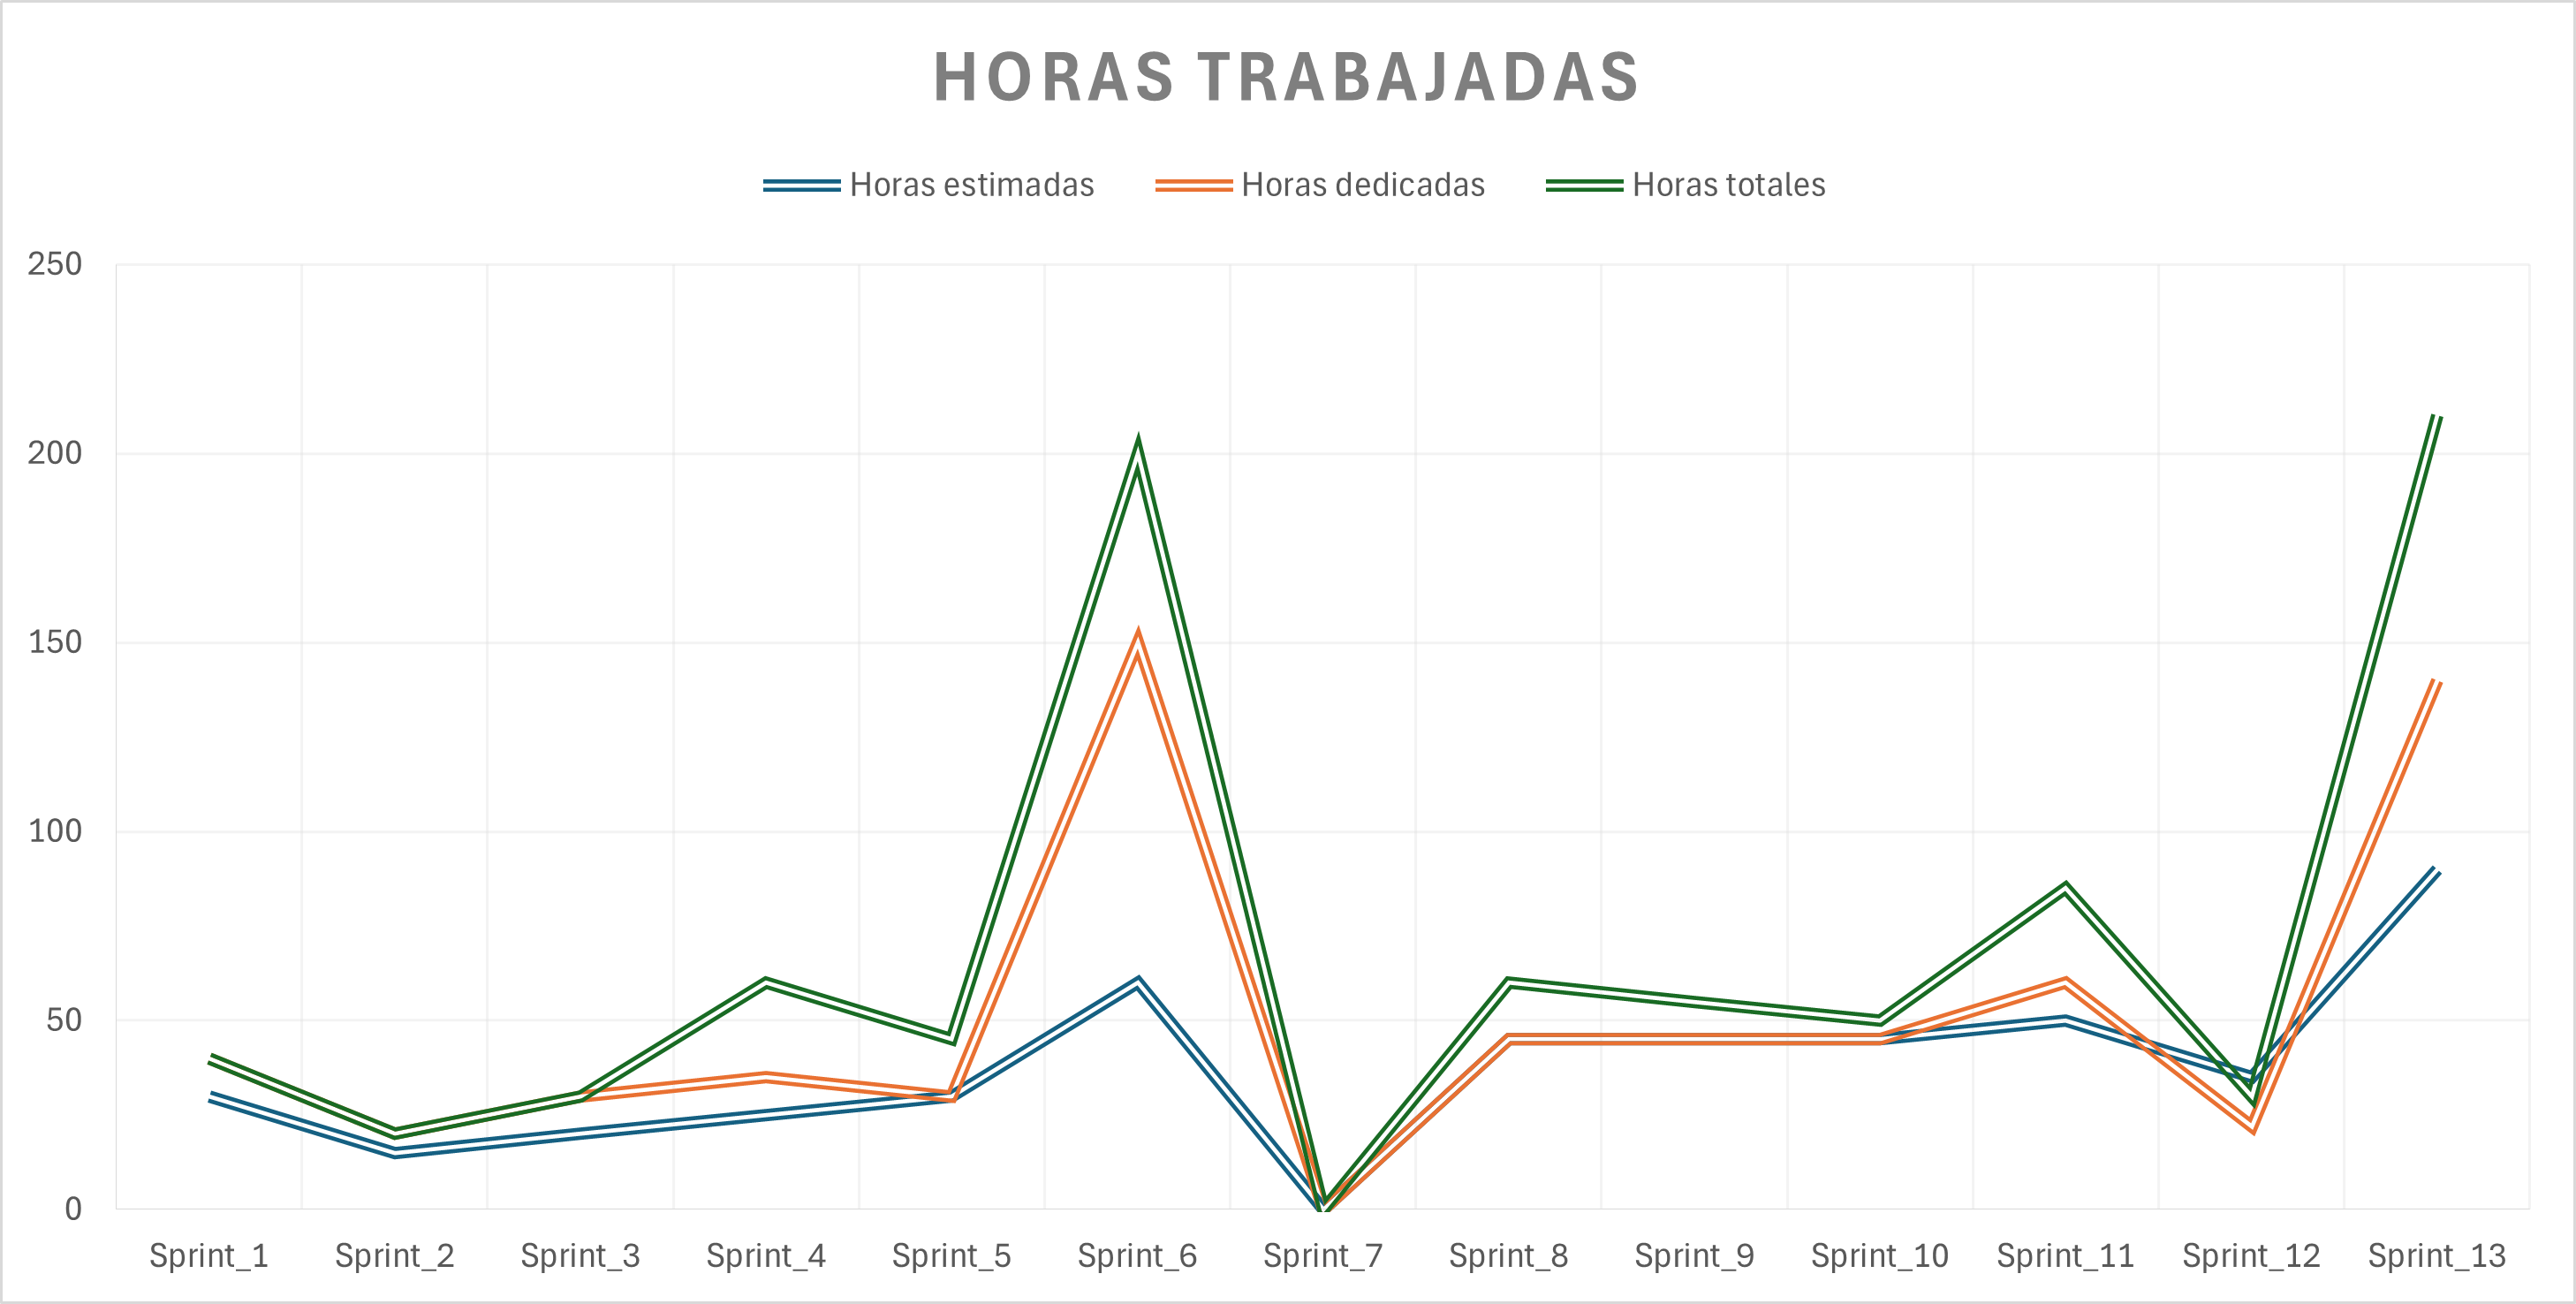
\includegraphics[width=1\linewidth]{img/horassprints.png}
    \caption{Gráfico de horas de sprints}
\end{figure}
\FloatBarrier

Como se observa en el gráfico, las horas estimadas fueron generalmente menores que las horas dedicadas, especialmente en las primeras fases del proyecto. Sin embargo, a medida que avanzó el desarrollo, las estimaciones se volvieron más precisas, reflejando un proceso de aprendizaje y mejora continua en la gestión del tiempo.

\section{Estudio de viabilidad}

En este apartado se analizará la viabilidad de este proyecto en un entorno profesional, evaluando los aspectos económicos y legales.

\subsection{Viabilidad económica}

La viabilidad económica es un aspecto absolutamente necesario en cualquier proyecto de software, ya que estos, para bien o para mal, suelen depender de los costes. Para este análisis se tomarán en cuenta todas las herramientas utilizadas, el coste profesional y el desgaste de los dispositivos empleados.

\subsection{Salarios}

Si este proyecto se hubiera llevado a cabo en una entidad privada, un ingeniero informático habría estado a cargo del desarrollo. El salario de este empleado dependería de la ubicación, el cargo y la experiencia. En este caso, tomaremos como referencia el salario medio bruto de un ingeniero informático en España. Según diversas fuentes como UAX, Bankinter y Talent.com, este ronda los 20.000 euros anuales para perfiles con poca experiencia.

Teniendo en cuenta que el proyecto consumió alrededor de \textbf{700 horas}, sin contar las horas de pruebas, el salario correspondiente sería de aproximadamente \textbf{6.731 euros}. 

Además, el trabajador podría enfrentarse a circunstancias imprevistas, como una baja médica, tal como ocurrió en este caso. Una situación así representaría un coste adicional para la empresa, que tendría que decidir entre sustituir al ingeniero durante la baja o postergar el proyecto. En España, durante una baja médica, el estado abona una parte del salario, mientras que la empresa debe cubrir otra. Si esta pausa hubiera durado 3 meses, el coste podría aumentar debido a la formación de un nuevo programador o la cobertura del sueldo de la baja si se asociara al proyecto.

\subsection{Hardware}

Otro coste adicional son los materiales utilizados. Aunque estos suelen durar más tiempo que el propio proyecto, deben ser amortizados anualmente. Para este análisis se aplicó una amortización de 5 años, es decir, el 20\% anual.

\begin{table}[H]
\centering
\begin{tabular}{lrr}
\toprule
Descripción & Coste Total & Amortización Anual \\ 
\midrule
Ordenador & 900€ & 180€ \\
Periféricos & 260€ & 52€ \\
Material de oficina & 20€ & 4€ \\
Imprevistos & 40€ & 8€ \\
\textbf{Total} & \textbf{1,220€} & \textbf{244€} \\ 
\bottomrule
\end{tabular}
\caption{Amortización de hardware y materiales.}
\end{table}

Durante el proyecto, pueden surgir imprevistos relacionados con el material. En este caso, uno de los componentes se averió y tuvo que ser sustituido.

\subsection{Software}

La mayoría de las herramientas de software utilizadas en este proyecto son de código abierto, por lo que no generan un coste adicional.

Sin embargo, el único servicio que sí representa un gasto es el proveedor de hosting para la página web, Render. Este cuenta con un plan gratuito, aunque no permite un despliegue sin interrupciones. Para evitar este problema, sería necesario optar por un plan de pago. 

El plan más económico cuesta aproximadamente 7€ mensuales, pero tiene capacidades limitadas. En contraste, el plan \textit{Pro Ultra}, que ofrece una mayor capacidad de cómputo adecuada para experimentos a gran escala, tiene un coste de 450€ mensuales. Para esta simulación, se considerará este último plan como el elegido, si se despliega los 3 últimos meses el precio seria de 1.350€ aunque este gasto seria periódico durante todo el tiempo que se quiera poner el servicio en funcionamiento.

Otras opciones que podrían haber sido evaluadas incluyen AWS o Azure. Sin embargo, para una evaluación adecuada sería necesario considerar factores como el uso esperado o el número de usuarios simultáneos.

\subsection{Gastos fijos}

Aunque el teletrabajo es común en la actualidad, muchas empresas continúan operando desde oficinas, lo que conlleva ciertos gastos fijos anuales.

\begin{table}[H]
\centering
\begin{tabular}{lr}
\toprule
Descripción & Coste Anual \\ 
\midrule
Internet y comunicaciones & 600€ \\
Electricidad y mantenimiento & 400€ \\
Limpieza & 1,000€ \\
\textbf{Total} & \textbf{2,000€} \\ 
\bottomrule
\end{tabular}
\caption{Gastos fijos estimados.}
\end{table}

Se han considerado los recursos básicos necesarios para garantizar un entorno funcional en una empresa informática.

\subsection{Costes y beneficios}

Finalmente, al calcular todos los costes, incluyendo los salarios, hardware, software y gastos fijos, se puede realizar una estimación global del coste del proyecto. A continuación, se presenta un desglose detallado:

\begin{table}[H]
\centering
\begin{tabular}{lr}
\toprule
Descripción & Coste \\ 
\midrule
Personal (Neto) & 6.731€ \\ 
Hardware (Amortización) & 244€ \\ 
Software (Servicios) & 1.350€  \\ 
Gastos fijos & 2,000€ \\ 
\textbf{Total Anual} & \textbf{10.325€} \\ 
\bottomrule
\end{tabular}
\caption{Resumen de costes del proyecto.}
\end{table}

El coste total estimado del proyecto se sitúa en torno a \textbf{10.325 euros}, considerando todos los aspectos mencionados.

En cuanto a los beneficios, estos dependerán del valor añadido que el proyecto pueda ofrecer a los usuarios finales y de la capacidad de la empresa para monetizar las funcionalidades desarrolladas. No obstante, este proyecto no está diseñado para una monetización directa. Su principal utilidad radica en su carácter experimental, proporcionando una base sólida para continuar con la implementación del algoritmo TRACLUS en diferentes ámbitos. Por tanto, su valor reside más en su potencial académico y como base tecnológica que en su rentabilidad económica inmediata.

\subsection{Viabilidad legal}

La viabilidad legal de un proyecto es un aspecto crítico, especialmente cuando se planea publicarlo para obtener un beneficio económico. Este análisis depende de las licencias asociadas a cada una de las herramientas y bibliotecas utilizadas durante su desarrollo.

A continuación, se presentan las herramientas y bibliotecas utilizadas, junto con sus licencias respectivas, así como una descripción de sus implicaciones legales.

\subsubsection{Herramientas}

\begin{table}[H]
\centering
\begin{tabular}{lr}
\toprule
Herramienta & Licencia \\ 
\midrule
Python 3.11.2 & PSF License (Python Software Foundation License) \\ 
Git & GNU General Public License v2.0 \\ 
Texmaker & GNU General Public License v2 \\ 
\bottomrule
\end{tabular}
\caption{Licencias de las herramientas utilizadas.}
\end{table}

\begin{itemize}
    \item \textbf{Python 3.11.2}  
        \begin{itemize}
            \item Licencia: PSF License (Python Software Foundation License).
            \item Características:
                \begin{itemize}
                    \item Permite usar, modificar y distribuir, tanto para proyectos abiertos como comerciales.
                    \item Compatible con licencias como la GPL.
                    \item Distribuido "tal cual", sin garantías.
                \end{itemize}
            \item Implicaciones: Asegura el acceso y uso de Python en proyectos de todo tipo.
        \end{itemize}

    \item \textbf{Git}  
        \begin{itemize}
            \item Licencia: GNU General Public License v2.0.
            \item Características:
                \begin{itemize}
                    \item Licencia copyleft fuerte que asegura que las modificaciones al código fuente sean abiertas y compartidas bajo la misma licencia.
                \end{itemize}
            \item Implicaciones: Es ideal para fomentar la transparencia en sistemas de control de versiones.
        \end{itemize}

    \item \textbf{Texmaker}  
        \begin{itemize}
            \item Licencia: GNU General Public License v2.
            \item Características:
                \begin{itemize}
                    \item Requiere que cualquier modificación o redistribución mantenga el código fuente abierto bajo la misma licencia.
                \end{itemize}
            \item Implicaciones: Garantiza que herramientas de edición de LaTeX sigan siendo accesibles para la comunidad.
        \end{itemize}
\end{itemize}

\subsubsection{Bibliotecas}

\begin{table}[H]
\centering
\begin{tabular}{lr}
\toprule
Biblioteca & Licencia \\ 
\midrule
Dash & MIT \\ 
Pandas & BSD \\ 
Matplotlib & Matplotlib License \\ 
Plotly & MIT \\ 
NumPy & BSD \\ 
sklearn.cluster & BSD \\ 
Shapely & BSD \\ 
PyProj & MIT \\ 
Contextily & BSD personalizada \\ 
\bottomrule
\end{tabular}
\caption{Licencias de las bibliotecas utilizadas.}
\end{table}

\begin{itemize}
    \item \textbf{Licencia MIT}  
        \begin{itemize}
            \item Características:
                \begin{itemize}
                    \item Permisiva: permite uso, modificación y redistribución incluso con fines comerciales.
                    \item Requiere incluir el aviso de copyright y la licencia original.
                \end{itemize}
            \item Implicaciones: Ideal para proyectos abiertos o comerciales.
            \item Usada por: Dash, Plotly, PyProj.
        \end{itemize}

    \item \textbf{Licencia BSD}  
        \begin{itemize}
            \item Características:
                \begin{itemize}
                    \item Permite uso y redistribución con atribución al autor original.
                    \item Existen dos versiones principales: BSD-2-Clause (simplificada) y BSD-3-Clause (que incluye restricciones adicionales para evitar promoción indebida).
                \end{itemize}
            \item Implicaciones: Muy permisiva y compatible con proyectos comerciales.
            \item Usada por: Pandas, NumPy, sklearn, Shapely, Contextily.
        \end{itemize}

    \item \textbf{Licencia Matplotlib}  
        \begin{itemize}
            \item Características:
                \begin{itemize}
                    \item Basada en la licencia BSD, permite uso y redistribución con atribución.
                \end{itemize}
            \item Implicaciones: Compatible con proyectos comerciales.
            \item Usada por: Matplotlib.
        \end{itemize}

    \item \textbf{Licencia Contextily (BSD personalizada)}  
        \begin{itemize}
            \item Características:
                \begin{itemize}
                    \item Similar a BSD, con ajustes específicos para el uso de datos abiertos y mapas.
                \end{itemize}
            \item Implicaciones: Garantiza libertad de uso y redistribución.
        \end{itemize}
\end{itemize}

\subsubsection{Conclusión}

En general, todas las herramientas y bibliotecas utilizadas en este proyecto están respaldadas por licencias permisivas que permiten su uso, modificación y distribución, incluso para fines comerciales. Sin embargo, para garantizar la viabilidad legal, es fundamental cumplir con los requisitos específicos de cada licencia, como la atribución de autoría en las licencias MIT y BSD, o la redistribución bajo la misma licencia en herramientas GPL como Git y Texmaker.

Esto asegura que el proyecto puede publicarse y distribuirse sin conflictos legales, siempre que se respeten las condiciones de las licencias asociadas.
